The convolution operation is a combination of concepts from the fcl and pooling.
Like in pooling, values get aggregated from inside a specific region of influence.
This region is called the \emph{kernel}.
They do however not get treated uniformly, but scaled with (learnable) weights before being summed up.
The weights are stored as entries in the kernel. 
The operation is equivalent to a the discrete mathematical 2D-convolution, however due to convention the kernel is flipped before the calculation in most mathematical definitions \cite{multidimConv} and is not flipped in most machine learning frameworks.
This has to be taken into account for non-symmetric kernels.
As for pooling, the sides are padded with zeros, if the input size is supposed to match to output size. 
An example convolution (un-padded) is calculated in \autoref{eq:convolution}, including the sample calculation for on of the values.

\begin{equation}
    \label{eq:convolution}
    \begin{split}
        \left(\begin{matrix}
            2 & \textcolor{blue}{-3} & \textcolor{blue}{1} & -4 \\
            1 & \textcolor{blue}{2} & \textcolor{blue}{1} & -2 \\
            -3 & 2 & -3 & 2 \\
            -1 & -1 & 1 & 4 \\
        \end{matrix}\right)\,\odot\,
        \left(\begin{matrix}
            1 & -1  \\
            2 & 1   \\
        \end{matrix}\right) = 
        \left(\begin{matrix}
            9 & \textcolor{blue}{y} & 5 \\
            -5 & 2 & -1 \\
            -8 & 4 & 1 \\
        \end{matrix}\right)\\
        y = (-3)\cdot 1 + 1 \cdot (-1) + 2 \cdot 2 + 1 \cdot 1 = 1
    \end{split}
\end{equation}

\paragraph{Full convolutions} are the kind of convolutions, for that the kernels \emph{channel} dimension $c$ matches the channel dimension of the input values.
Images - that are one of the primary targets for convolutions - typically have not only a width and a height, but also a channel dimension (typically color channels, like rgb).
Because of that, images are typically stored as 3D-tensors ($c \times h \times w$).
A 3D-convolution with a ($c \times o \times k_h \times k_w$) kernel, produces an output of shape ($o \times h \times w$) (with appropriate padding, that is always assumed from this point onward).
The dimension $o$ can be seen as the number of kernels, that get independently applied and later stacked.
The leftmost case in \autoref{fig:comparison-depthwise-convolution} shows such a convolution with $h = w=8,\, k_h =k_w = 3,\, c = 3 \mathrm{\,and\,} o=1$.

\begin{figure}[htbp]
    \centering
    \makebox[\textwidth][c]{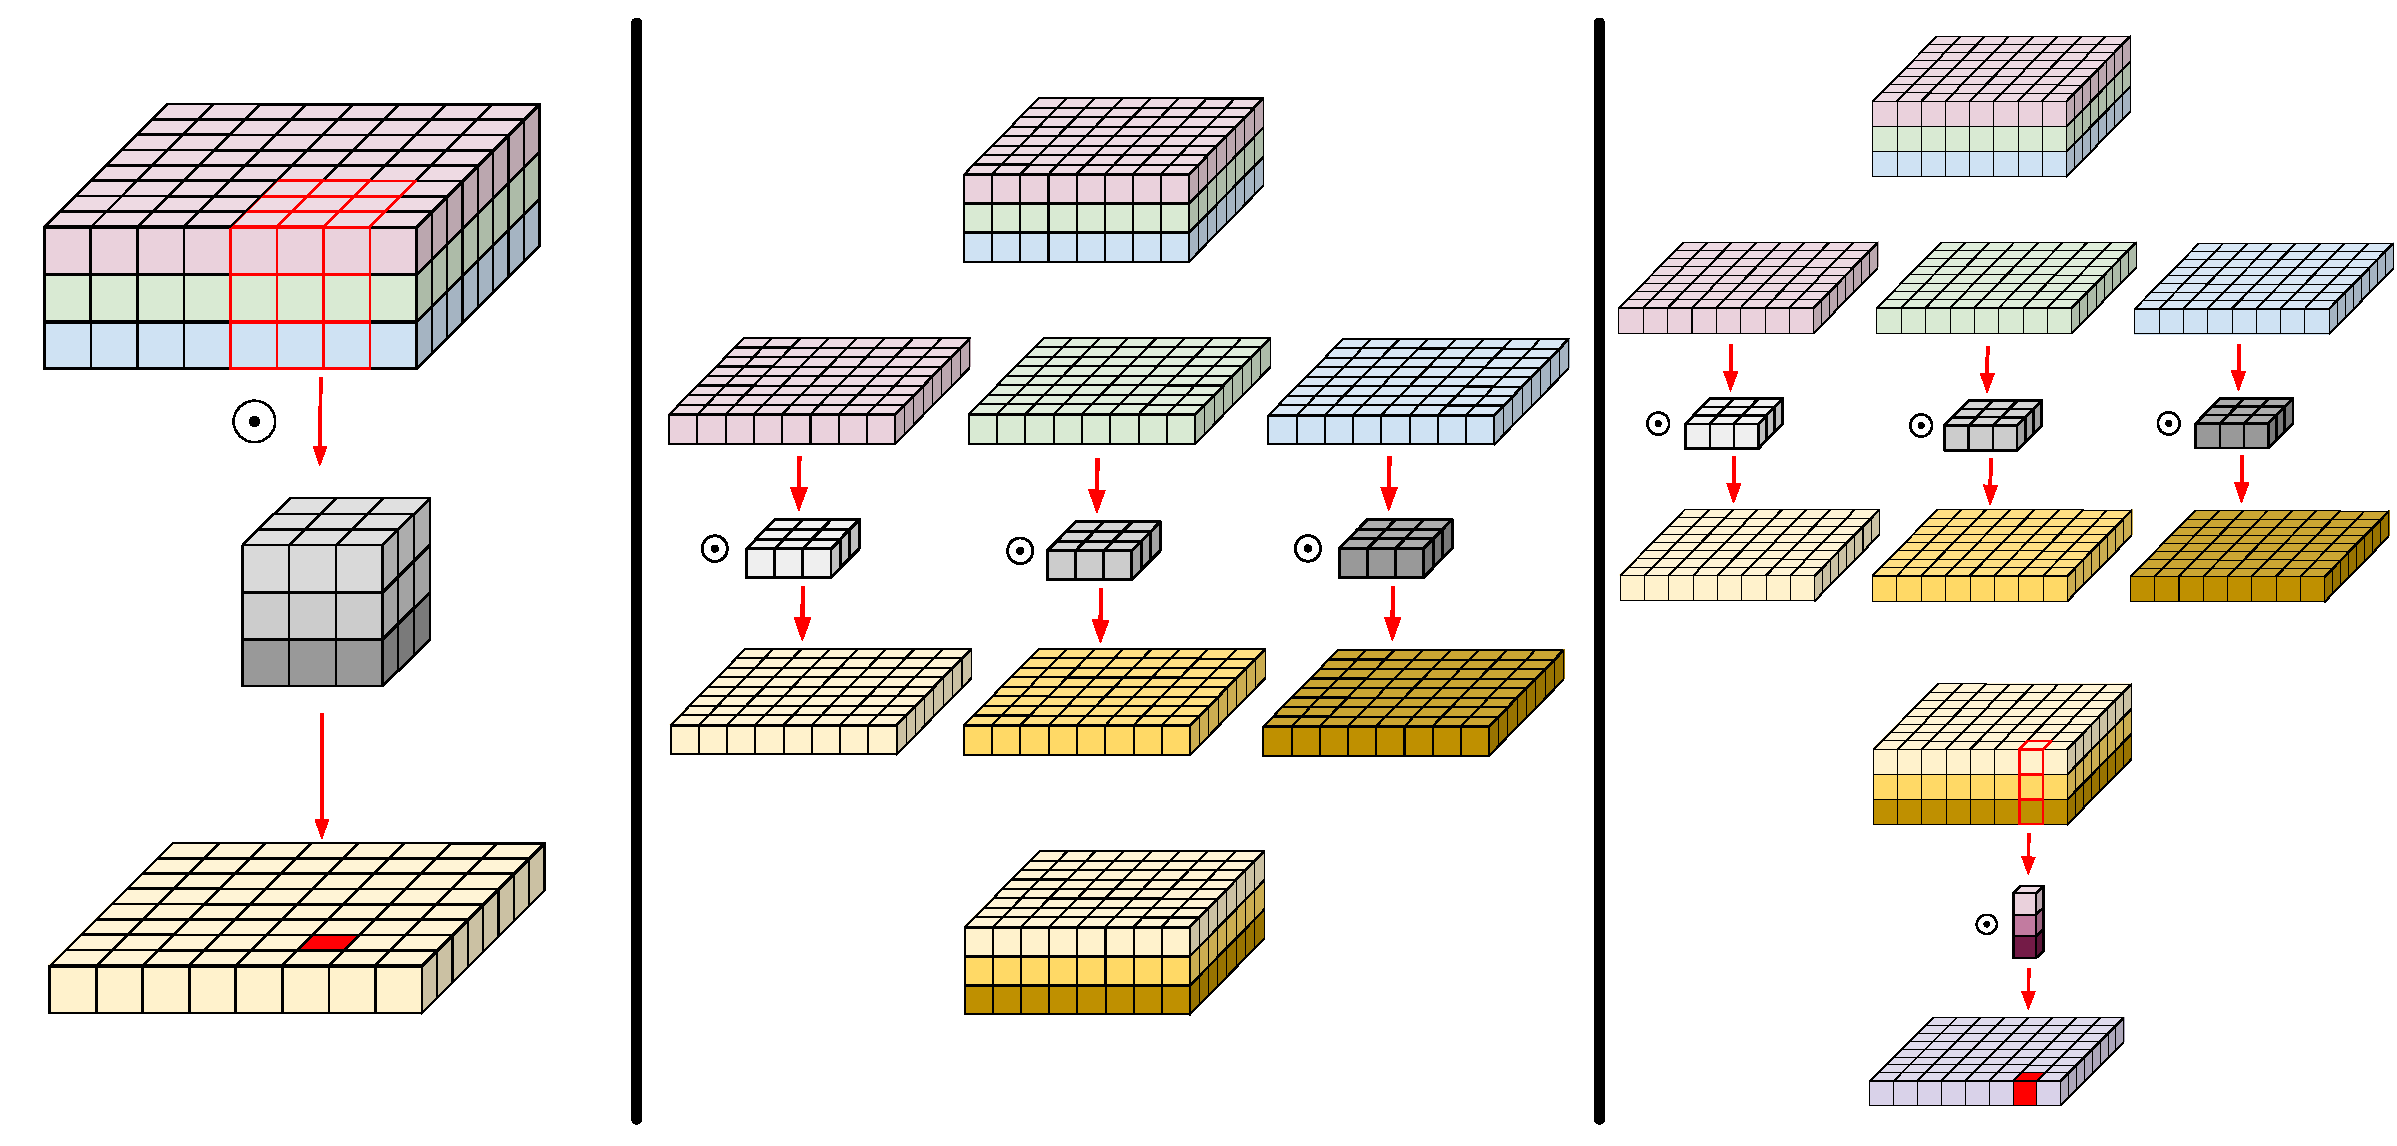
\includegraphics[width=1.1\textwidth]{./architectures/theory/convolutions/depthwise.pdf}}
    \caption{This figure show the differences between a \emph{normal convolution} (left), a \emph{depthwise convolution}  (center) and a \emph{depthwise separable convolution} (right).
    The normal convolution has a 3D-kernel. The depthwise convolution splits this into multiple 2D-kernels.
    The depthwise separable convolution works basically in the same way as the depthwise, but at the end a 1D-kernel (1$\times$1-convolution) is used to combine the channels.
     Original image from \cite{separableConvolutions}, but modified and almost completely redrawn.}
    \label{fig:comparison-depthwise-convolution}
\end{figure}

\paragraph{Depthwise convolutions} are similar to full convolutions at a first glance (such a convolution is pictured in the center of \autoref{fig:comparison-depthwise-convolution}).
They employ an independent ($1\times 1 \times k_h \times k_w$) kernel for each channel and stack their results.
The output channel count $o$ can only be a whole number multiple of the input channel count (one in the figure, but it is easy to use for example two filters per channel).
Other groupings of channels are possible \cite{channelNets}.
By itself, this model computes no interaction across input channels. 
This seems like a disadvantage, but in reality is exact what will be needed for the construction of \emph{strict convolution based metaformer} (see \autoref{sec:architectures-metaformer}).

\paragraph{Depthwise separable convolutions} are the logical continuation to depthwise convolutions and were made popular in image processing neural networks with the introduction of the \emph{MobileNets} \cite{mobileNetPaper}.
They get rid of two limitations of the depthwise convolutions: the number of output channels can be chosen freely and the information exchange is not limited to the channels in isolation.
This is done by following up the ($1\times 1 \times k_h \times k_w$) convolutions with ($c \times o \times 1 \times 1$) convolution, that brings the number of output channels $o$ up to any desired number ($o =1$ on the right side of \autoref{fig:comparison-depthwise-convolution}).
The advantage is the reduction of the kernel size. This makes for easier computation and smaller model storage footprints. 
The weight count is compared in \autoref{table:weight-count-convolutions}.

\begin{table}[htbp]
    \centering
    \makebox[\textwidth][c]{
        \begin{tabular}{l|ccc} 
            \toprule
            Convolution Type    & Formula \#weights & \# for $o=6,\,c=3,$   & \# for $o=6,\,c=6,$ \\  
                                                &   & $k_h=k_w=3,\,s=3$     & $k_h=k_w=4,\,s=4$     \\  
            \midrule 
            full                & $o\cdot (c\cdot k_h\cdot k_w)$                                & 162  & 576 \\
            depthwise           & $(o//c) \cdot c\cdot (1\cdot k_h\cdot k_w)$                   & 54   & 96 \\
            depthw. separable   & $c\cdot (1\cdot k_h\cdot k_w) + o \cdot (c \cdot 1 \cdot 1)$  & 45   & 132 \\
            full symm.          & $o\cdot (c\cdot s)$                                           & 54   & 144 \\
            depthwise symm.     & $(o//c) \cdot c\cdot (1\cdot s)$                              & 18   & 24 \\
            depthw. sep. symm.  & $c\cdot (1\cdot s) + o \cdot (c \cdot 1 \cdot 1)$             & 27   & 60 \\
            \bottomrule
        \end{tabular}
    }
    \vspace{0.2cm}
    \caption{Comparison of the number of weights needed for the different convolution types.
            $o$ is the number of output channels, $c$ the number of input channels, $k_h$ and $k_w$ denote the kernel size and $s$ is the number of different tracked distance-weights in a symmetric case.
            Note that the depthwise symmetric case is always the most efficient in terms of the number of parameters. 
            This is also the case, that gets employed in the metaformer, because there the mixing across channels is actually not needed (depthwise separable and full convolutions provide that mixing).
            For $o>>c$, the depthwise separable convolution will always require less weights than the depthwise.
            }
    \label{table:weight-count-convolutions}
\end{table}

\paragraph{Symmetric convolutions} are a further extension to the convolution concept. 
They employ \emph{shared weights} in the kernel.
That means not every kernel element need to be stored separately.
An example for a typical $3\times 3$ symmetric kernel is shown in \autoref{eq:symmetric-convolution}. 

\begin{equation}
    \label{eq:symmetric-convolution}
    \left(\begin{matrix}
        \textcolor{textyellow}{w_2} & \textcolor{textgreen}{w_1} & \textcolor{textyellow}{w_2}\\
        \textcolor{textgreen}{w_1} & \textcolor{textred}{w_0} & \textcolor{textgreen}{w_1}\\
        \textcolor{textyellow}{w_2} & \textcolor{textgreen}{w_1} & \textcolor{textyellow}{w_2}\\
    \end{matrix}\right)
\end{equation}

This $3\times 3$ kernel only needs three weights to be stored. 
While implementing the forward pass for such kernels is trivial, it is not quite obvious how to achieve an efficient calculation of the error gradient needed for the backpropagation to work.
Implementations of symmetric cases exists \cite{symmetricConvolutionImplementation}, but not in the same format as \autoref{eq:symmetric-convolution}.
The error values from convolutions also get computed through a convolution operation \cite{backpropagationInConvolutions}. 
The machine learning frameworks probably perform convolution backpropagation way more efficient, than it was possible to implement the mathematics to propagate the correct error term into the shared weights by hand.

As a solution, the convolution kernel can be assembled from multiple kernels that can be scaled individually and added after the convolution is performed for each of them.
This computes the correct convolution and can be backpropagated by the frameworks by default.
The calculation is shown in \autoref{eq:how-to-compute-symm-conv}.

\begin{equation}
    \label{eq:how-to-compute-symm-conv}
    \begin{split}
        \overleftrightarrow{X} &\,\odot\, \left(\begin{matrix}
            \textcolor{textyellow}{w_2} & \textcolor{textgreen}{w_1} & \textcolor{textyellow}{w_2}\\
            \textcolor{textgreen}{w_1} & \textcolor{textred}{w_0} & \textcolor{textgreen}{w_1}\\
            \textcolor{textyellow}{w_2} & \textcolor{textgreen}{w_1} & \textcolor{textyellow}{w_2}\\
        \end{matrix}\right) = \\
        \textcolor{textred}{w_0}\cdot \overleftrightarrow{X} \,\odot\, \left(\begin{matrix}
            0&0&0\\
            0&1&0\\
            0&0&0\\
        \end{matrix}\right)+
        \textcolor{textgreen}{w_1}\cdot \overleftrightarrow{X} &\,\odot\, \left(\begin{matrix}
            0&1&0\\
            1&0&1\\
            0&1&0\\
        \end{matrix}\right)+
        \textcolor{textyellow}{w_2}\cdot \overleftrightarrow{X} \,\odot\, \left(\begin{matrix}
            1&0&1\\
            0&0&0\\
            1&0&1\\
        \end{matrix}\right)
    \end{split}
\end{equation}


The implementation of the symmetric (depthwise) convolution for images can be found at \cite{selfComputerScience}, \filepath{/models/helpers/SymmConv2d.py}.